\documentclass[12pt]{article}
%\usepackage{paper} %if the document does not compile properly for you on the initial build, uncomment \usepackage{paper} and build again. This should force MikTeX to install package "paper"
\usepackage[margin=1in]{geometry}
\usepackage{float}
\usepackage{natbib}
\bibliographystyle{apsr}
\usepackage{graphicx}
\graphicspath{ {../fig/} }
\usepackage{setspace}
\setstretch{2}
\usepackage[super]{nth}
\usepackage{booktabs}
\usepackage{makecell}

%\usepackage{hyperref}
%\usepackage{etoolbox}
%\AtBeginEnvironment{quote}{\singlespacing\small}

\begin{document}

\title{First Year Paper:\\ \large{\citet{iyengar2012affect}}}
\author{Robert Lytle}
\date{\today}
\maketitle
\thispagestyle{empty}
\clearpage
\section{Introduction}
The question ``Has the mass public polarized alongside elites?" has been the subject of an enormous amount of scholarly debate. This debate has been held largely in terms of ideology, with scholars leveraging competing evidence showing \citep{abramowitz2010disappearing} or not showing \citep{fiorina2012disconnect} mass-level polarization. \cite{iyengar2012affect} argue that affect (one's emotional valence towards a stimulus) rather than ideology should be used to evaluate levels of mass polarization. The authors leverage a variety of publicly available observational datasets
 (further discussed in the body of this work) to demonstrate that Democrats and Republicans exhibit increasing animosity towards out-partisans. In this paper, I replicate the findings of \cite{iyengar2012affect} as they relate to the effect (or lack thereof) of policy preferences on affective polarization, and extend the original work by including respondents' status as primary voters in the model. I expect to find that policy preferences have a greater effect on out-party affect among primary voters than their non-voting counterparts.


\section{Summary of \cite{iyengar2012affect}}
\textit{Affect, Not Ideology} is an ambitious work; seeking to describe the historical trends of affective polarization and to establish a causal chain between hostile media, party-ID, and mass-level affective polarization. This analysis is done in service of the authors' central argument: that Americanist scholars of polarization should study the attitudes of voters towards members of the out-party, not just the ideological differences between opposing parties.

The vast majority of scholars have evaluated polarization in terms of divergent policy preferences between parties and their supporters and have produced contradictory results. While virtually all agree that \textit{elites} have become more polarized, some argue this elite polarization is in response to an increasingly polarized \textit{public} \citep{abramowitz2010disappearing} and some argue against the notion of mass polarization altogether \citep{fiorina2012disconnect, fiorina2005culture}. Still other scholars have argued that observed polarization is not the result of increasingly extreme policy positions on the part of Democrats and Republicans, but the result of previously ideologically heterodox partisans sorting themselves into more appropriate parties \citep{levendusky2009partisan}.

Each of the works discussed in the previous paragraph share a common focus on partisans' \textit{ideology}. Iyengar, Sood, and Lelkes identify this commonality and argue that, since most people have a limited conception of their own ideology \citep{converse1964nature}, and tend to have conflicting \citep{mcclosky1984american} and ideologically incoherent views \citep[p. 76--96]{zaller1992nature}, ideological differences are not a suitable metric by which to gauge mass polarization. In the view of the authors, partisans' affect towards their opponents is a more consistent and substantively meaningful diagnostic of the degree of mass polarization.

To demonstrate this, the authors leverage several existing survey datasets and an advertising dataset\footnote{\textit{ANES Cumulative Study, YouGov/Polimetrix 2008 Election Study}, a \textit{YouGov 2011 multi-national study, Almond \& Verba (1960), Blair Center Election Study}, an \textit{AP Yahoo! News 2008} Election Study and the \textit{Wisconsin Advertising Project}. The implications for validity in using survey data will be discussed in greater detail in section 3.}. The survey data are used first to describe the degree of affective polarization, and are then used in conjunction with the advertisement data to establish a causal link between exposure to hostile political media and affective polarization. Survey data from the United Kingdom is included in the descriptive portion of the research, intended by the authors to serve as a pseudo-control for country-level effects \citep[p. 407]{iyengar2012affect}, comparing a country with parties whose ideology is more salient (the U.K.) to the U.S.

The authors find evidence supporting their claim that the U.S. has undergone a large increase in affective polarization, while the U.K. has polarized ``only modestly" (p. 417) since the 1960s. Further, they find little evidence to suggest the animosity in the U.S. is driven by ideological differences between partisans, contending instead that the ``mere act of identifying with a political party is sufficient to trigger negative evaluations of the opposition" \citep[p. 407]{iyengar2012affect}. They further find support for their claim that exposure to hostile media campaigns strengthens individuals' partisan convictions \citep[p. 407]{iyengar2012affect}, though problems with their finding will be discussed in Section 3.3 of this paper. Finally, they close the paper by reiterating their call for a broader investigation of affect by scholars.

In short: \citeauthor{iyengar2012affect} identify a shortcoming in the ongoing debate over the existence of mass-level polarization---that scholars have focused exclusively on partisans' ideology. Instead, they argue that analyses of ideology are insufficient means by which to evaluate mass polarization. The authors argue for a new conception of division: partisans' affect towards their opponents. Iyengar et al. show that partisans are becoming increasingly divided from (and hostile towards) one another and posit that this division is the result of increasingly hostile media, rather than ideological differences between partisans. Therefore, ideological homogeneity between Democrats and Republicans is not sufficient evidence of a broader lack of polarization.



\subsubsection{Authors' Model of Affective Polarization}
The core hypothesis (\textit{\textbf{H1}}) of Iyengar et al. is that the U.S. is subject to increasing levels of affective polarization. This polarization, by definition, is dependent \textit{exclusively} on individual level animus towards out-partisans. Working backwards up the causal chain, animus towards the outparty is caused by salient partisan identity (\textit{\textbf{H2}}). The salience of party ID is then increased by politically charged media (\textit{\textbf{H3}}). This chain is represented in \textit{Figure \ref{fig:dag}'s} Directed Acyclic Graph (DAG) by the nodes ``Party ID" and ``Individual-level Out-party Animus" each of which can be both an outcome or exposure variable, depending on the hypothesis in question.

While the descriptive claim \textbf{\textit{H1}} is articulated clearly in the text, the presentation of the causal claims is more muddled; this becomes a problem when attempting to draw causal inferences from the data. These issues result from an imprecise translation of the theoretical data-generating process to statistical causal inference, and are discussed further in Section 3.3.6.

\begin{figure}[h!]
\center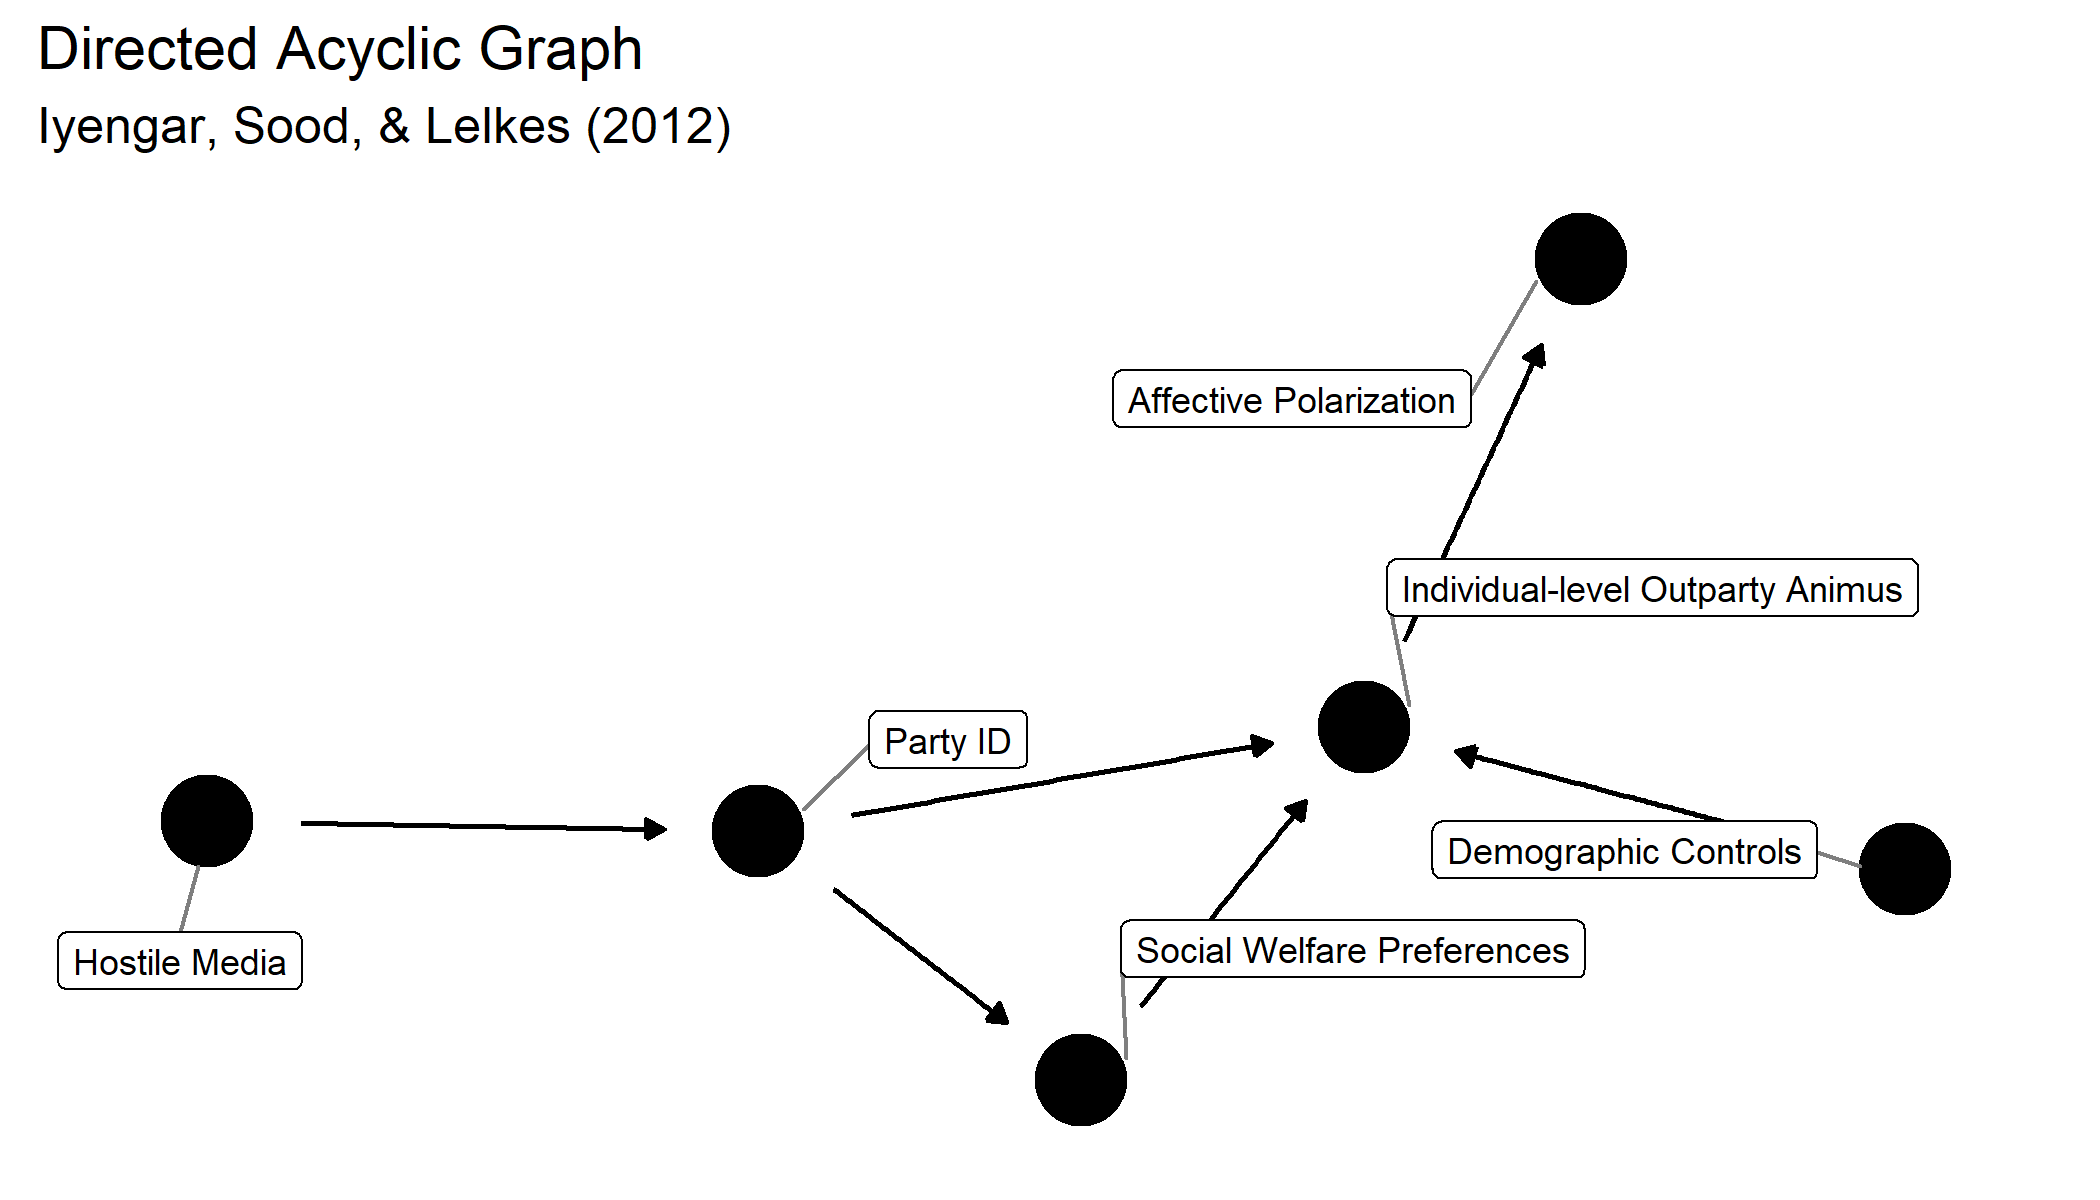
\includegraphics[width=6in]{ext-dag.png}
\caption{\label{fig:dag}\textit{A Directed Acyclic Graph of the causal processes described by \citeauthor{iyengar2012affect}.}}
\end{figure}

Fortunately, the core descriptive claim is both sound and a valuable contribution to the polarization literature. Iyengar et al. show unambiguous and increasingly wide attitudinal cleavages between supporters of the major parties, using a previously under-explored set of measures. While the authors' causal model is flawed, they succeed in showing the existence of a phenomenon which \textit{can} be modeled.

Still, there is more work to be done even on the descriptive front. This study does not address sub-partisan units of political identity, such as self identification as a member of a specific caucus or faction (e.g. progressive, tea-party, alt-right) within the broader party and the implications these identities may have for animus directed at an outgroup. A subgroup analysis along these lines is proposed in Section 4.



\subsection{Research Design Concerns and Limitations}

\subsubsection{Validity and Reliability}
\citeauthor{iyengar2012affect} operationalize inter-partisan affect using two principal measures. The first, ``net partisan affect" (NPA), is the difference between partisans' rating of their in-party and out-party on a feeling thermometer (p. 411). This measure is supplemented with respondents' answer to the question: 
\begin{quote}
``How would you feel if you had a son or daughter who married a Republican/Democrat (Conservative/Labor) supporter? Not at all upset, somewhat upset, very upset?" (p.411)
\end{quote}
Both of these measures are high in content validity, but should still be treated with some caution, dependent as they are on self-assessed survey data. First, it is not clear the degree to which the authors' measures of mass polarization are actually picking up antipathy towards party supporters or party \textit{elites}. The marriage question above clearly asks about ``supporter(s)", but the ANES feeling thermometers are more ambiguous, asking respondents to describe ``people who are Republicans or Democrats" \citep[p. 412]{iyengar2012affect}. In this second example, the elite status of the fictional Republican or Democrat is not specified, and it may not be clear to the respondent (or researcher) what sort of Republican or Democrat the respondent described.

Second, surveys are notoriously vulnerable to issues of framing, priming, and response instability \citep[p. 53--75]{zaller1992nature}, which at best introduce noise in the data and at worst (or at the most interesting, depending on one's perspective) are illustrative of a broader problem with the measurement of public opinion---that many people are simply ``Making it up as [they] go along", to borrow a phrase from Zaller. While these problems are not addressed by \citeauthor{iyengar2012affect} \textit{post facto}; surveys (including the ANES, from which much of these data are drawn) take steps to ameliorate some of the threat from other forms of response bias, often randomizing the order in which questions are asked so as to avoid priming respondents. Still, the larger problem of instability is a more fundamental problem, and one that is not addressed in the text.

A third validity concern of these data is the possibility that respondents have under reported their attachment to their party. As people generally express a preference for bipartisanship \citep{harbridge2014public}, there is logical reason to believe respondents' desire to appear less partisan could lead to Hawthorne effects or social-desirability bias, posing a potential threat to the construct validity of the findings \citep[p. 73, Table 3.1 Item 8]{shadish2002experimental}. Fortunately, if the results are the product of social desirability bias they should \textit{underestimate} the degree of affective polarization. Thus the possibility of unaccounted for social desirability bias does not pose a major threat to the core findings of the paper.


\subsubsection{Unit of Analysis}

\citeauthor{iyengar2012affect} use individual level attitudinal data to make inferences about the state of the broader population. Their primary hypothesis is that the United States exists in an increasingly affective polarized state---a condition which is only possible to achieve through the individual attitudes of many individuals. Referring to the DAG presented in \textit{Figure \ref{fig:dag}}, we see that polarization is wholly dependent on individual out-party animus. In this case it is perfectly legitimate to draw mass level inferences from individual level data.

\subsubsection{Manipulability \& Randomization}

Party ID is difficult to manipulate in an observational study. It is conceivable that an experimental design could assign participants a particular party ID in the limited context of that experiment, but given the importance of individuals’ actual party ID there would be reason to doubt the external validity of such a study. 

Media exposure can be more easily manipulated in an experimental setting, as in \citet{mutz2007effects}, but the external validity of such experiments is questionable, given the differences between media consumption in the laboratory and in more complex information environments. Fortunately, the opportunity to conduct a natural experiment outside of the laboratory environment exists.

Iyengar et al use residence in a ``battleground state"\footnote{Defined by the authors as ``States with the two parties’ vote difference of less than 5 percent in the 2000 elections...FL, IA, MO, MN, NH, NM, NV, OH, OR, PA, and WI".} as the exposure variable in their regression to capture the effect of hostile media on partisans' affect (p. 424). Greater causal leverage could be gained over the effect of media by instead conducting a natural experiment using a Geographic Regression Discontinuity (GRD) design. Campaign ads are purchased and distributed in ``Designated Market Areas (DMAs)", collections of counties in which a television ad is shown. These DMAs may extend across multiple states \citep{keele2015geographic}. In other words: residents of a non-battleground state $A$ may reside in a DMA which largely services a battleground state $B$. Residents of the DMA in state $A$ will be exposed to the ads targeting state $B$. Residents of state $A$ living outside the DMA will not be exposed to battleground ads.

In such a GRD design, state $A$ counties in state $B$'s DMA are considered the treatment group, while state $A$ counties \textit{adjacent} to the DMA are considered the control. While individuals likely self-select into states, it is unlikely that residents self-select into particular DMAs \textit{within} those states. Extant scholarship has exploited this as-if random assignment in the study of media and voter turnout \cite{krasno2008televised, huber2007identifying}.





%Designated Media Exposure



\subsubsection{Implicit Counterfactuals}
The implicit counterfactual, a condition of weak partisan identity, is not necessarily unrealistic but is \textit{unlikely}. The salience of partisan identity appears to be at a historical high, and the trend does not appear poised to level out any time soon. Still, some researchers have demonstrated experimental interventions which seem to decrease the importance of party ID to participants (Levendusky, Forthcoming). Additionally, both major parties seem to be undergoing a period of increased ideological heterogeneity, with the left and moderate wings of the Democratic party seemingly ascendant and the embrace of Trump by many (but not all) elites in the Republican party. Scholars have argued that internal ideological heterogeneity was a sufficient condition for the (relatively) low salience of party ID through much of the 20th Century \citep{rohde1991parties}; as such, there is reason not to entirely discount the possibility of a return to an era of relatively weak party ID.

%\subsubsection{SUTVA}
%The Stable Unit Treatment Value Assumption (SUTVA) is the assumption that one individual receiving (or not) the treatment condition does not not affect the outcome in other individuals in the study---the effect of $x$ on $i_1$ is the same, regardless of if (or how) individuals $i_2 \ldots i_n$ received the treatment \citep[p. 48]{morgan2015counterfactuals}. 
%SUTVA is violated in this model, with the potential for spillover effects between partisans. While posing problems for causal inference, this SUTVA violation is intrinsic to the study of polarization. Polarization, by definition, implies an in-group and an outgroup; the compositions of which influence the attitudes of the other. 

%The outcome we are interested in is the social distance between individuals $d_n$ and $r_n$ in groups $D$ and $R$. We can expect this effect to vary based on the treatment homogeneity of $D$ and $R$. In other words, the effect produced by one individual’s partisan identity can depend on the identities and the strength of those around her. For a group identity to be salient (and therefore to produce a powerful effect on social distance towards an outgroup) we would expect to find heterogeneity in the outgroup and homogeneity in the ingroup \citep{rohde1991parties}. As noted by the authors of this study (and authors of more recent work) the observed increase in affective polarization has been concomitant with elite-level partisan sorting over the 20th and 21st centuries. 

\subsubsection{Endogeneity \& Confounders}


While the \textit{central} hypothesis of this study is largely descriptive, the DAG describing the data-generating process of \citeauthor{iyengar2012affect} is complex---containing several other potential problem areas. The DAG confusion arises because several of the nodes are both exposure and outcome variables. For example, in \textbf{\textit{H2}} party ID is the exposure variable, whereas it is an outcome in \textbf{\textit{H3}}. The authors' theory holds that the media affects affective polarization \textit{only} through its effect on party ID (p. 407), yet the party ID variable is included in the regression equation for media exposure on partisan affect, suggesting possible over control bias.

There are two possibilities:
\begin{enumerate}
\item The theory is correct, and the effect of media has been underestimated due to controlling for a node  in the middle of a causal path \citep{elwert2014endogenous}.
\item The theory needs to be amended; media effects partisan affect in ways that are not predicated on an increased sense of party ID.
\end{enumerate}
In addition to this concern, there is the possibility of over control bias when evaluating the effect of policy preferences on affect, as policy preferences are often endogenous to party ID \citep{druckman2013elite}\footnote{This is also acknowledged in the footnotes on page 422 of \citeauthor{iyengar2012affect}.}. This case is not alarming however, as party ID was not included as a variable when regressing affect on policy preferences. While the authors' articulation of their causal claim is problematic, their core descriptive claim (that the United States has increasingly affectively polarized since the mid-\nth{20} century) is unaffected by these problems.

\section{Suggested Extensions}
\subsection{Subgroup Analysis}
I would like to conduct a subgroup analysis stratifying partisans by the candidate they supported in presidential primaries. The vast majority of polarization research treats party-ID as the ``least common denominator" of political identity. While party ID is clearly deeply important to voters' identities, I suspect that meaningful differences between members of party factions may go unnoticed when examining the party holistically---both in terms of faction members' affect, and the role ideology plays in shaping that affect. I argue that primaries are a convenient tool for assessing these factional differences for a variety of reasons.

 First, primaries are an opportunity for ideological differences between co-partisans to become salient. While ideology may be only loosely related to affect toward the out-party there is a relationship between social-welfare preferences and inter-party animus \citep[p. 423]{iyengar2012affect}. Second, the effect of policy preferences on net partisan affect is more pronounced among the politically engaged (who are more likely to participate in primaries). Third, there are qualitative similarities between expressions of political identity in primary and general elections; primary voters wear shirts, display bumper stickers and post yard signs proclaiming their preferred candidates, just as they do in general elections. In addition to partisans' identities as  ``Republicans" or ``Democrats" they may have salient sub-identities as a ``Ron Paul" or ``Bernie Sanders" supporters.
 
Because primary voters tend to be more politically engaged, I hypothesize that ideology will be a stronger predictor of affect towards both the out-party and the in-party among primary voters. Further, as the primaries present a rare opportunity for individuals to express approval or dissatisfaction with the parties performance, I suspect that the net partisan affect of primary voters (and non-voters) will vary by their candidate of choice. Below, I present evidence of affective \textit{and} ideological differences between groups of primary voters and non-voters.


 \begin{table}[h!]
\begin{table}[H]
\centering
\begin{tabular}{ll>{\raggedleft\arraybackslash}p{3cm}>{\raggedleft\arraybackslash}p{3cm}>{\raggedleft\arraybackslash}p{3cm}>{}p{3cm}>{}p{3cm}>{}p{3cm}}
\toprule
\textbf{Year} & \textbf{Vote Choice} & \textbf{Net Partisan Affect} & \textbf{Dem Affect} & \textbf{Rep Affect}\\
\midrule
2008 & Didn't Vote & 47.43 & 78.55 & 31.76\\
2008 & Hillary Clinton & 48.37 & 76.51 & 28.14\\
2008 & Barack Obama & 53.63 & 80.40 & 26.77\\
2016 & Didn't Vote & 45.80 & 71.99 & 28.60\\
2016 & Hillary Clinton & 60.19 & 82.62 & 22.48\\
\addlinespace
2016 & Bernie Sanders & 48.34 & 67.70 & 21.45\\
\bottomrule
\end{tabular}
\end{table}
\caption{\label{table} \textit{Average net partisan affect, feeling thermometer towards the Democrat and Republican Parties, and self assessed ideology, reported across primary voters. Other candidates have been excluded due to very low $n$. These data are filtered by party-ID; all respondents are Democrats (leaning independents have been excluded)
.}}
\end{table}

Table 1 displays data from the 2008 and 2016 ANES: showing the net partisan affect, feeling thermometer towards each party and self assessed ideology of Democrats after the 2008 and 2016 primaries. Each value is averaged across vote choice. In these simple descriptive statistics we see substantial differences between supporters' in-party affect in both 2008 and 2016 in terms of net partisan affects. Notably, the differences in NPA between Sanders and Clinton supporters in 2016 are the product of coldness towards the \textit{in}party on the part of Sanders supporters, rather than any warmth towards the Republicans. These data suggest that the author's claim that ``in-party affect has changed little over time" (p. 412) belies heterogenous in-party affect between subgroups of co-partisans. To be sure, partisans are still much warmer toward their in-party than their out-party, but this is more true for some groups than others. 

A thorough subgroup analysis would necessarily include both Republicans and Democrats and extend farther back than the 2008 primary. In light of potential data availability concerns--the ANES only inconsistently asks primary vote choice questions--these analyses could be supplemented with time series study of the \textit{variation} of in-party affect and NPA. These analyses would be relatively straightforward to conduct, and would illuminate an underdeveloped segment of the polarization literature.

%\begin{figure}[H]
%\center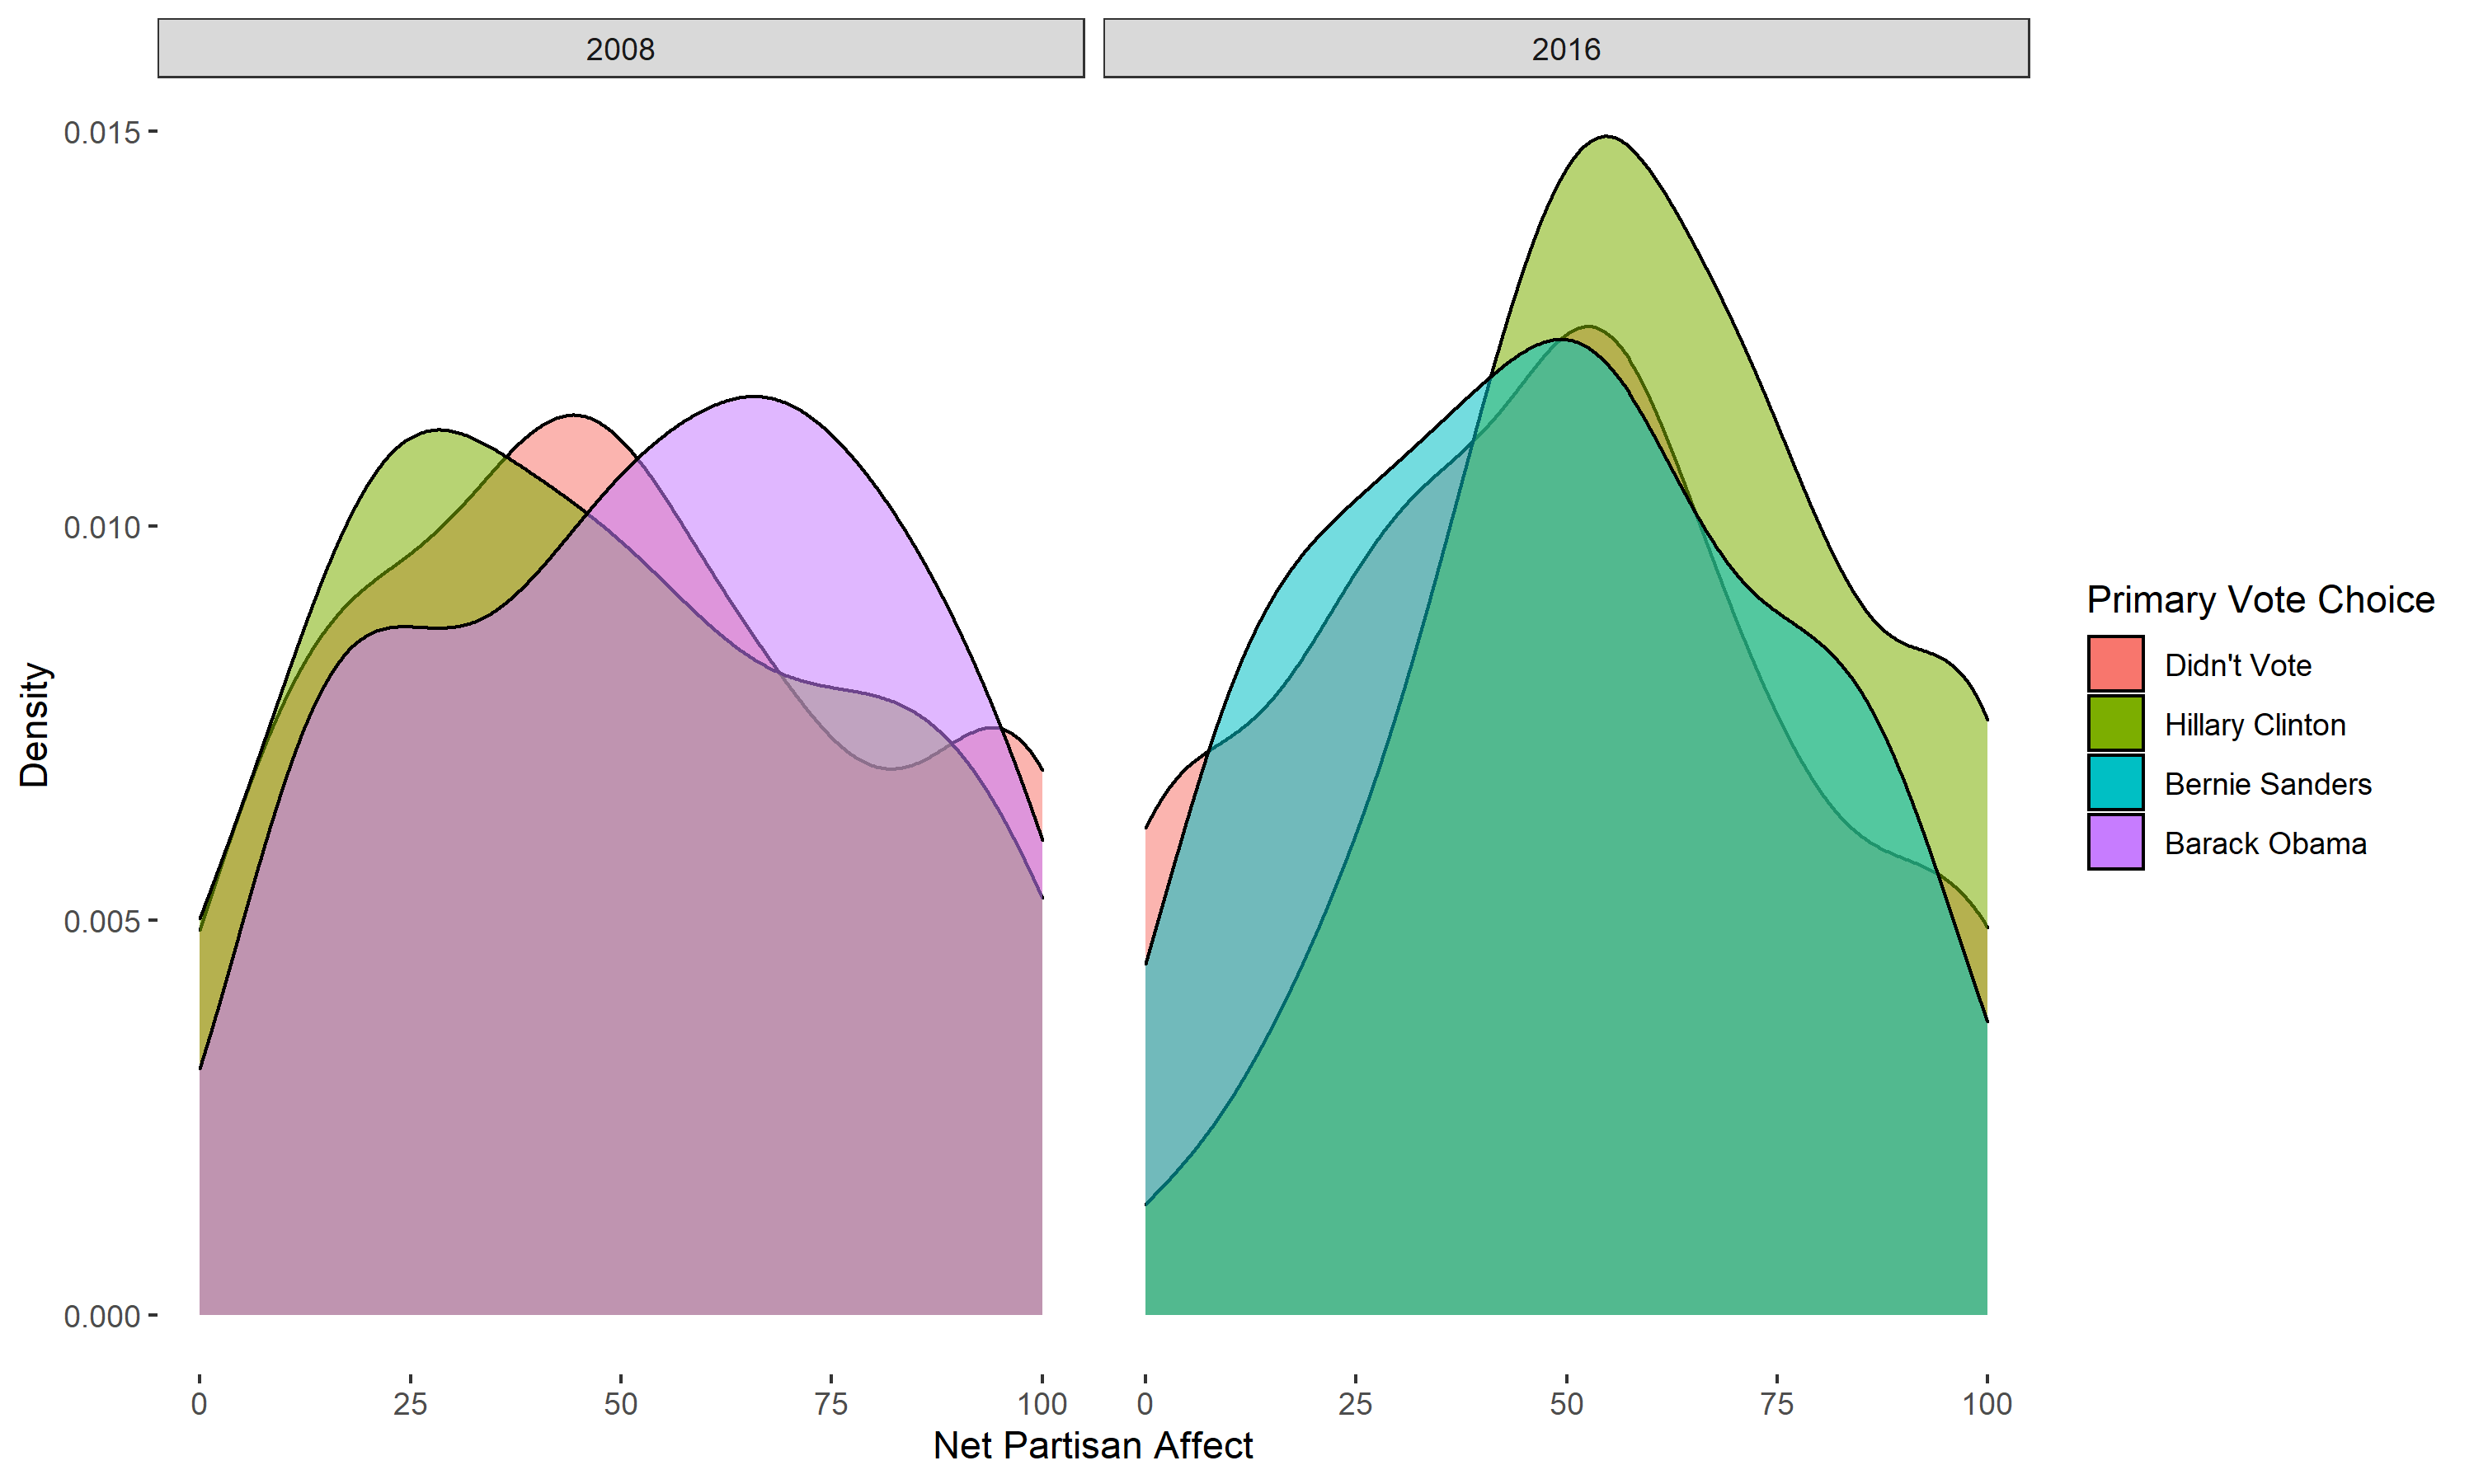
\includegraphics[width=6in]{therm-hist-2016.png}
%\caption{\label{fig:dens}\textit{Density plots of net partisan affect by vote in primary elections}.}
%\end{figure}

%These data are obviously quite limited, looking at members of one party across two years, but they should motivate additional research.


%compare decrease in NPA of losers to average NPA decrease of losers.

%Any observational evaluation of ideological strength is problemmatic because most self-assessments of ideology are typically one-dimensional---asking respondents for their ideological position, but not their \textit{commitment to} that position. Investigating activism may be a useful work-around to this problem. While activists tend to be more extreme than non activists, it would be foolish to believe that \textit{all} activists are more extreme than \textit{all} non-activists. Given these features of ideology, it would be particularly valuable to examine differences in affective polarization between activists and non-activists of similar ideology scores.


\thispagestyle{empty}
\clearpage
\setstretch{1}
\bibliography{references}

\end{document}

%